\documentclass{article}
\usepackage[a4paper,left=1in, right=1in, top=1in, bottom=1in]{geometry}
\usepackage{hyperref}
\usepackage{graphicx}
\usepackage{wrapfig}
\usepackage{subcaption}
\usepackage{comment}
\usepackage{array}
\usepackage{longtable}
\DeclareGraphicsExtensions{.pdf,.png,.jpg}
\graphicspath{ {./images/} }

\begin{document}
\title{Gibbot v5 PCB}
\author{Andrew Griesemer}
\maketitle
\tableofcontents
\newpage
\section{dsPIC Pinout}
\begin{figure}[h!]

	\centering
	\begin{subfigure}{0.4\textwidth}
		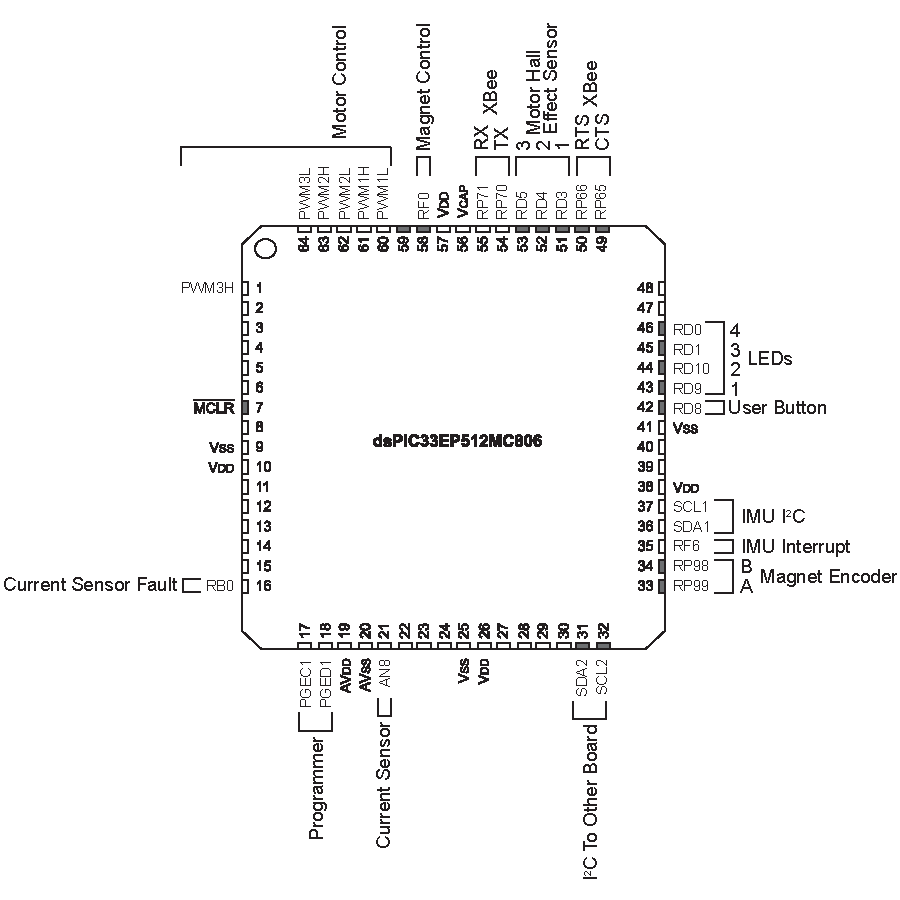
\includegraphics[width=\textwidth, page=1]{breakout}
		\label{pinout1}
	\end{subfigure}
	\begin{subfigure}{0.4\textwidth}
		\includegraphics[width=\textwidth, page=2]{breakout}
		\label{pinout2}
	\end{subfigure}
	\caption{ (a) pin assignments for primary board (b) pin assignments for secondary board}
\end{figure}

\section{Power Regulation}
The board is powered by a 24V power cable.  
\begin{figure}[h]
	\centering
	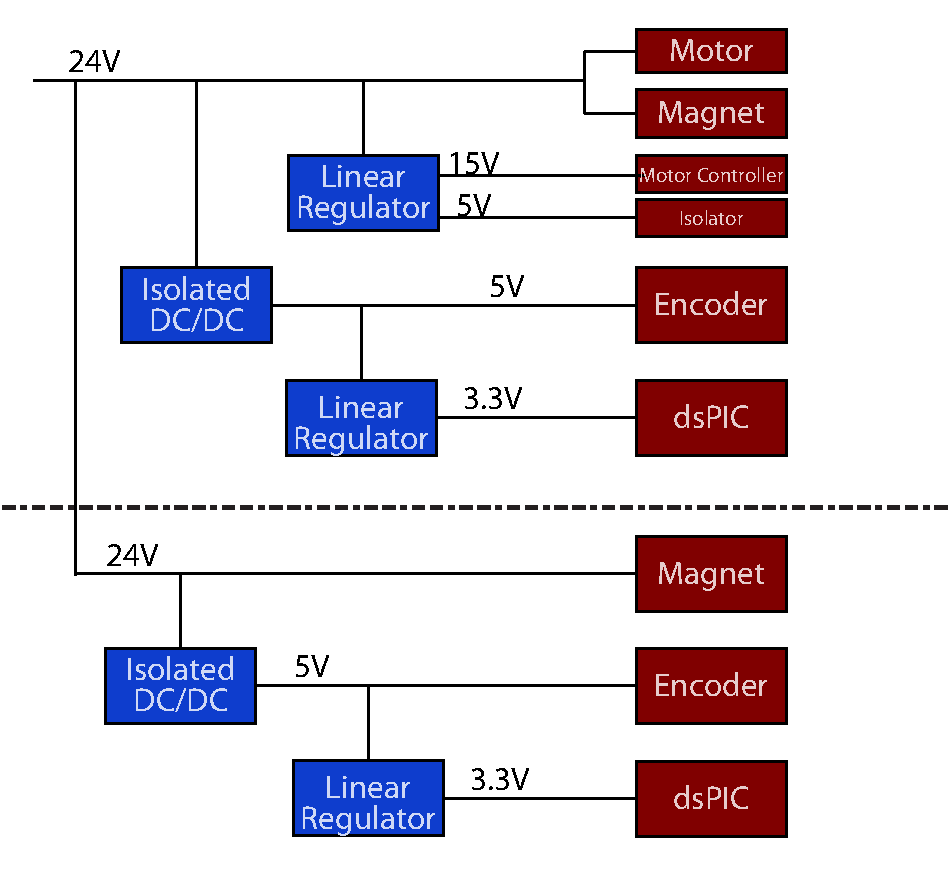
\includegraphics[width=.5\textwidth]{V5PowerPath}
	\label{powerpath}
	\caption{Flowchart of power planes}
\end{figure}
\subsection{Primary Board}
\subsubsection*{24V}
\begin{longtable}{|c | c | c |  >{\centering\arraybackslash}p{0.4\textwidth} |} \hline
Component & Current per unit & Total Component & Source of Current Value\\ \hline
EM237-24-212 Magnets & 230mA x 2 & 460mA & Current at rated voltage \footnote{APW Catalog http://catalog.apwcompany.com/Asset/6489.pdf}\\ \hline
EC 60 Flat Motor & & $<10$A & Control specification\\ \hline
\end{longtable}
\subsubsection*{15V}
\begin{longtable}{|c | c | c |  >{\centering\arraybackslash}p{0.4\textwidth} |} \hline
Component & Current per unit & Total Component & Source of Current Value\\ \hline
2 Encoders & 78mA x 2 & 156mA & 62mA maximum no load current + 8mA x 2 maximum output current\footnote{E3 1800 CPR product page http://www.usdigital.com/products/e3}\\ \hline
\end{longtable}
\subsubsection*{5V}
\begin{longtable}{|c | c | c |  >{\centering\arraybackslash}p{0.4\textwidth} |} \hline
Component & Current per unit & Total Component & Source of Current Value\\ \hline
E3 Encoders & 78mA x 2 & 156mA & 62mA maximum no load current + 8mA x 2 maximum output current\footnote{E3 1800 CPR product page http://www.usdigital.com/products/e3}\\ \hline
\end{longtable}
\subsubsection*{3.3V}
\begin{longtable}{|c | c | c |  >{\centering\arraybackslash}p{0.4\textwidth} |} \hline
dsPIC && 320mA & Absolute maximum rating current from VSS\footnote{dsPIC33EP512MC806 datasheet http://ww1.microchip.com/downloads/en/DeviceDoc/70616g.pdf}\\ \hline
Status LEDs & 3.3mA x 6& 20mA & Assuming 3.3V and 1k resistor\\ \hline
IMU && 10mA & 3.9mA gyro + 6mA magnetometer\footnote{MPU-9150 datasheet http://dlnmh9ip6v2uc.cloudfront.net/datasheets/Sensors/IMU/PS-MPU-9150A.pdf} \\ \hline
IR LEDs &10mA x 6 & 60 mA & 3.3V  and 330 ohm resistor\\ \hline
\textbf{Total} && \textbf{0.410 A} &\\ \hline
\end{longtable}
\addtocounter{table}{-4}  % Decrement table counter so that first table is labeled as Table 1

\subsection{Digital Isolation}
In previous iterations noise from the motor caused spurious errors across the board. To eliminate the noise the V5 board uses a \href{http://www.digikey.com/product-search/en?vendor=0&keywords=CC6-2405SF-E}{CC6-2405SF-E} isolated DC/DC converter on each board to isolate the 5V ground plane from the 24V ground plane. Digital signals to the motor controller and the magnet MOSFETs are transmitted through \href{http://www.digikey.com/product-detail/en/SI8610EC-B-IS/336-2058-5-ND/2623300}{SI86x0EC-B-IS1} series digital isolators.

\newpage
\section{BLDC Motor Driver}
\subsection{BLDC Motor Background}
A Brushless DC Motor is different from a brushed DC motor because it lacks the internal brushes that allow a typical DC motor to reverse the direction of current flow as the rotor coil rotates within the magnetic stator. In order to drive a BLDC motor the direction of current flow must be commutated by external control circuitry. Benefits of BLDC motors over brushed motors include lighter weight for the same amount of torque and increased longevity.

A typical BLDC motor has two or more coils and a sensor that can determine the angular position of the rotor. A microcontroller reads the state of the sensor and changes the direction of current across the coils in order to maximize torque. The BLDC motor on the Gibbot is the Maxon EC 60 Flat which has 3 coils and 3 Hall Effect sensors that detect the angular position of the rotor. A commutation pattern diagram is shown in Figure \ref{fig:commutation}. This diagram depicts the same pattern as the diagram in the Maxon E-Paper Catalog\footnote{\raggedright Figure \ref{fig:commutation} is taken from pg 32 of the Maxon E-Paper Catalog http://epaper.maxonmotor.ch/en/}, but has been modified for clarity. In the diagram the binary hall effect sensor states are shown on top. The MOSFET bridge outputs are shown below. The MOSFET bridge states are indicated as either high, low or float. The float state is represented by a diagonal line. 
\begin{figure}[h!]
	\centering
	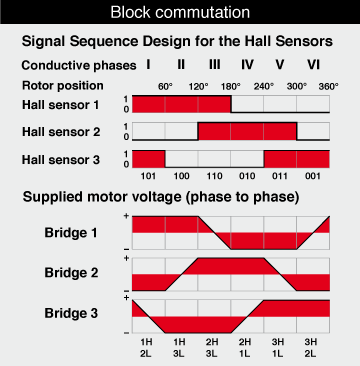
\includegraphics[width=0.4\textwidth]{commutation2}
	\caption{The commutation pattern for the Maxon EC 60 Flat Motor.}
	\label{fig:commutation}
\end{figure}

The pin connections for the Maxon EC 60 Flat motor hall effect sensor ribbon cable  are given in Table \ref{tab:motpin1}a. Note: The pin numbering from the EC 60 Flat catalog page is for a ribbon cable that has been replaced. The motor pole connections are given in Table \ref{tab:motpin1}b.

\begin{table}[h!]
	\centering
	\caption{Motor Connections}
	\begin{subtable}[t]{0.4\textwidth}	
		\centering
		\subcaption{Hall Effect Cable Pin Connections}
		\begin{tabular}{| c | c | c |}
			\hline
			\textbf{Color} & \textbf{Pin Number} & \textbf{Connection} \\ \hline
			Blue & 1 & 5V \\ \hline
			Gray & 2 & GND \\ \hline
			Gray & 3 & 1 \\ \hline
			Gray & 4 & 2 \\ \hline
			Gray & 5 & 3 \\ \hline
		\end{tabular}
	\end{subtable}
	\begin{subtable}[t]{0.4\textwidth}
		\centering
		\subcaption{Motor Pin Connections}
		\begin{tabular}{| c | c |}
			\hline
			\textbf{Color} & \textbf{Pin Connection} \\ \hline
			Red & 1  \\ \hline
			Black & 2 \\ \hline
			White & 3 \\ \hline
		\end{tabular}
	\end{subtable}
	\label{tab:motpin1}
\end{table}

For a lower power application the control of each coil of the motor could have been accomplished by a typical H-bridge. Because the Gibbot requires up to 10A at 24V the commutation circuitry requires higher power H-bridges using MOSFETs.  Figure~\ref{fig:hbridge} shows the schematic of an H-bridge connection for a single coil. The pull down resistor on the low-side MOSFET gate prevents both MOSFETs from activating before the dsPIC turns on. 

\begin{figure}[h]
	\centering
	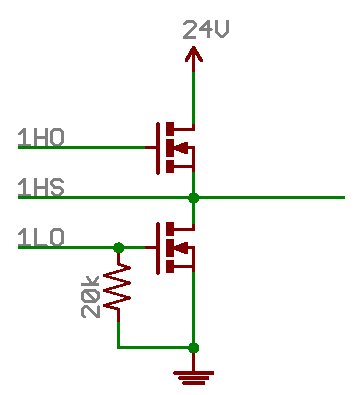
\includegraphics[width=0.3\textwidth]{hbridge}
	\caption{A single H-bridge for the BLDC motor}
	\label{fig:hbridge}
\end{figure}

\subsection{HIP4086 Driver}
The driver circuit uses Intersil's HIP4086 3-Phase MOSFET driver\footnote{Datasheet http://www.intersil.com/content/dam/Intersil/documents/hip4/hip4086-a.pdf}. This chip solves two issues with driving the MOSFETs from a dsPIC, (1) stepping up the control voltage for the low side MOSFET from the microcontroller's logic level 3.3V to the 15V required to fully turn on the MOSFET. (2) stepping up the gate voltage for the high side MOSFET to 15V plus the motor drive voltage. This voltage level is required because the high side MOSFET's source is connected to the motor coil so the gate-to-source voltage on the high side MOSFET is referenced to the motor voltage. The HIP4086 accomplishes this higher voltage with Bootstrap capacitors (more info in Section \ref{sec:bootstrap}). The chip also has added functionality such as programmable deadtime which is described further in Section \ref{sec:deadtime}.

\subsection{MOSFET Selection}
The bridge MOSFETs are the most critical components in the BLDC driver. The MOSFETs must be able to switch quickly and withstand the high drive voltages and switching currents. 
\begin{description}
\item[Gate Charge ($Q_G$)] The switching speed of the MOSFET is primarily determined by the gate charge. A smaller gate charge correlates with faster switching time so the gate charge should be minimize. The gate charge listed on a datasheet is typically the gate charge at a $V_{GS}= 5V$ . However, when the HIP4086 has a supply voltage of 15V $V_{GS}$ will be 15V. To determine $Q_G$ at this voltage a plot of $Q_G$ vs $V_{GS}$ is used. The plot from the datasheet of the MOSFETs used in the current motor driver circuit, the IRFR3806TRPBF, is shown in Figure \ref{fig:qg}\footnote{\raggedright IRFR3806PbF datasheet pg 3 http://www.irf.com/product-info/datasheets/data/irfr3806pbf.pdf}. From the plot $Q_G$ = 33nC at $V_{GS}$=15V
\begin{figure}[h]
	\centering
	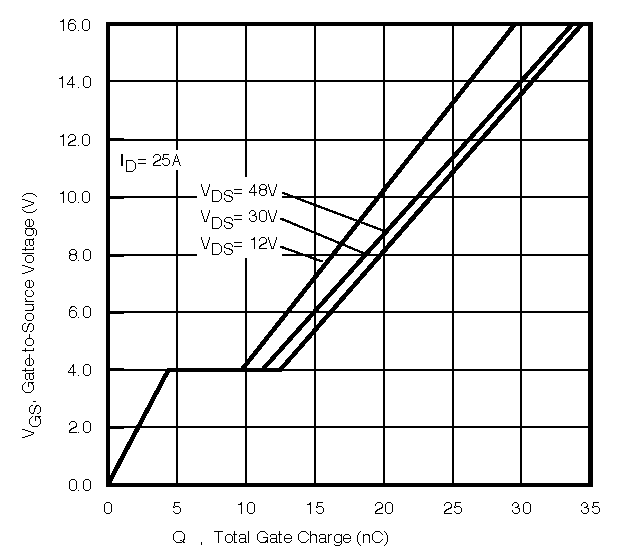
\includegraphics[width=0.4\textwidth]{qg2}
	\caption{Typical Gate Charge vs. Gate-to-Source Voltage linearly extrapolated to $V_{GS}=15V$.}
	\label{fig:qg} 
\end{figure}


\item[Max Continuous Current]
The required continuous current for the motor to achieve the desired torque is 10A. 
\item[Max Drain to Source Voltage ($V_{DS}$)] The required drain-to-source voltage is the same as the Motor Supply Voltage, which was 48V, but is now 24V. To keep the design flexible to the higher voltage range $V_{DS}$ is set a value above 48V. 
\item[Max Gate-to-Source Voltage ($V_{GS}$)] The required gate-to-source voltage is determined by the gate drive voltage of the HIP4086 driver. This gate drive voltage is the same as the supply voltage for the HIP4086. The recommended maximum operating supply voltage on the HIP4086 datasheet\footnote{\raggedright HIP4086 Datasheet pg 5 http://www.intersil.com/content/dam/Intersil/documents/hip4/hip4086-a.pdf} is 15V. To keep the design flexible to supply voltages for the HIP4086 the max gate-to-source voltage should be at least $\pm15V$. 

\item[On State Drain-to-Source Resistance ($R_{DS(ON)}$)] The on state resistance effects the efficiency of the drive circuitry and partially determines the temperature rise during operation. $R_{DS(ON)}$ should also be minimized.

 \item[Maximum Power Dissipation ($P_D$)] This value is not considered in MOSFET selection. While the ability of the MOSFET to dissipate heat from conducting is important, the way in which $P_{D,MAX}$ is defined varies widely between manufacturers. Moreover, the ability of a MOSFET to dissipate heat should not vary significantly between different devices in the same physical package. Determining a specification for power dissipation would also be difficult because it involves a combination of the power dissipated during turn-on and turn-off periods when $R_{DS}$ is high and the power dissipated during the fully on state at the much lower $R_{DS(ON)}$.
\end{description}

\subsection{Clamping Circuit}
The HIP4086 Datasheet and the HIP4086 Demo Board User Guide provide two different methods of clamping the HS pin to prevent negative transients. The two methods are shown in Figure \ref{fig:clamping}. The purpose of the clamping circuit is to limit the negative transient voltage that is induced when the high side MOSFET is turned off to the -6V voltage limit specified for the HIP4086. The two methods accomplish this while limiting the current that is able to flow through the path during the deadtime when both MOSFETs are off. The method used in the HIP4086 Datasheet (Figure \ref{fig:clamping}a) uses two diodes in series.  The method used in the HIP4086 Demo Board User Guide (Figure \ref{fig:clamping}b) uses a single diode with a resistor in series. Because values are not established for the resistor in the Demo Board User Guide method we used the simpler method from the Datasheet (Figure \ref{fig:clamping}a).
\begin{figure}[h]
	\caption{Alternate clamping circuitry from the HIP4086 documentation\protect\footnotemark.}
	\label{fig:clamping}
	\centering
	\begin{subfigure}{0.5\textwidth}
		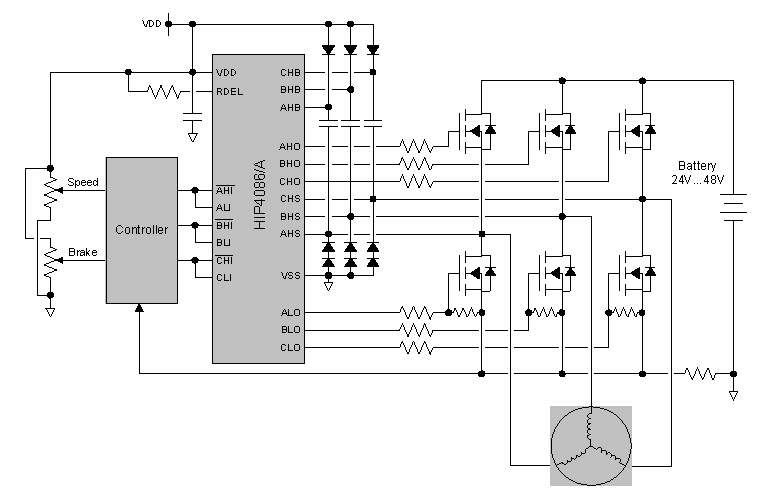
\includegraphics[width=\textwidth]{clamp1}
		\caption{HIP4086 Datasheet}
	\end{subfigure}
	\quad
	\begin{subfigure}{0.35\textwidth}
		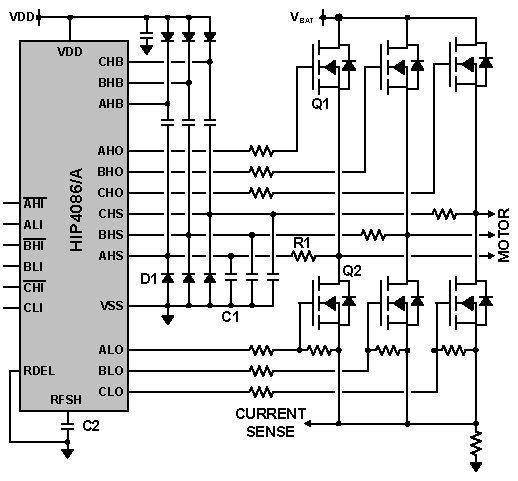
\includegraphics[width=\textwidth]{clamp2}
		\caption{HIP4086 Demo Board User guide}
	\end{subfigure}	
\end{figure}

\footnotetext{HIP4086 datasheet pg 12 http://www.intersil.com/content/dam/Intersil/documents/hip4/hip4086-a.pdf and HIP4086 Demo Board User Guide, Application Note 1829 pg 7 http://www.intersil.com/content/dam/Intersil/documents/an18/an1829.pdf}

\subsection{Bootstrap Capacitor, Diode and Resistor Selection}
\label{sec:bootstrap}
The boot capacitor value is chosen so that the capacitor can provide the gate charge of the driven FET without causing the capacitor voltage to sag excessively. 

The formula for calculating bootstrap capacitance from the HIP4086 datasheet is:

\[Q_C = Q_{GATE} + Period \cdot \left ( I_{HB} + \frac{V_{HO}}{R_{GS}} + I_{GATELEAK} \right )\]

Because there is no gate-to-source resistor for the high side MOSFETs, the $\frac{V_{HO}}{R_{GS}}$ term can be eliminated. The other values are calculated as follows:\\

$Q_{GATE}$ = 32nC, gate Charge of the MOSFET at $V_{GS}=15V$ and $V_{DS} \approx 30V$ from Figure \ref{fig:qg}.

$Period$ = 50$\mu$s, maximum on time of the high side MOSFET at 100\% Duty Cycle.

$I_{HB}$ = 100$\mu$A, worst case high side current through the xHB pin of the HIP4086.

$I_{GateLeak}$ = 100nA, leakage current of the MOSFET gate.

\[Q_C = 32nC + \frac{1}{20,000Hz}*(100uA + 100 nA) = 37nC\]

\[C_{BOOT} = \frac{Q_C}{Ripple \cdot V_{DD}} \]
\[C_{BOOT} = \frac{37nC}{5\% \cdot 15V} = 49nF \approx 0.047uF\]


\subsection{Set Dead Time on the HIP4086}
\label{sec:deadtime}
Because the gate capacitance of the MOSFET keeps the MOSFET on for a period of time after the control signal has gone low, there must be a delay between the turn-off event of one PWM
output in a complementary pair and the turn-on event of the other. Otherwise shoot through might occur when both MOSFETs are conducting causing the power to short to ground. The time between transitions of the control PWM signal is called dead time. In the current configurations of the Gibbot dead time is redudantly programmed into both the dsPIC PWM control as well as the HIP4086. 

Dead time on the HIP4086 is set using a resistor between ground and the pin $R_{DEL}$ on the HIP4086. Figure \ref{fig:deadtime} from the HIP4086 datasheet can be used to set $R_{DEL}$ approximately.
\begin{figure}[h]
	\centering
	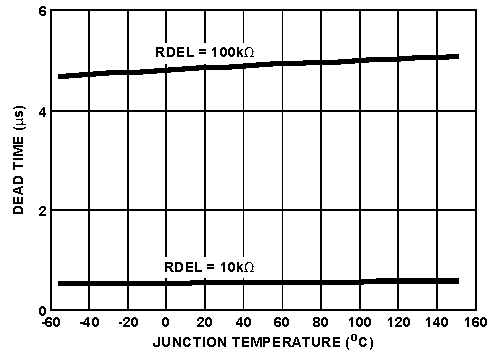
\includegraphics[width=0.5\textwidth]{deadtime}
	\caption{ $R_{DEL}$ vs. Dead Time\protect\footnotemark}
	\label{fig:deadtime}
\end{figure}
\footnotetext{\raggedright From HIP4086 3-Phase Bridge Driver Configurations
and Applications pg 4 \href{http://www.intersil.com/content/dam/Intersil/documents/an96/an9642.pdf}{http://www.intersil.com/content/dam/Intersil/documents/an96/an9642.pdf}}

\section{Inertial Measurement Unit - MPU9150}
The MPU9150 is a 9-axis sensor with a 3-axis gyroscope, a 3-axis accelerometer and a 3-axis magnetometer. There is an MPU9150 on both the primary and secondary board. The supporting circuitry is shown in Figure \ref{mpu9150} below\footnote{MPU9150 
Product Specification p21 http://www.invensense.com/mems/gyro/documents/PS-MPU-9150A-00v4\_3.pdf}. Pull-up resistors in a 0402 package are attached the the SCL and SDA I\textsuperscript{2}C communication lines. 

\begin{figure}[h!]
	\centering
	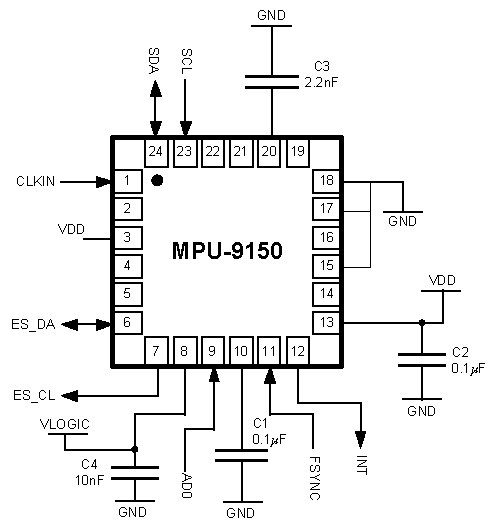
\includegraphics[width=0.4\textwidth]{mpu9150}
	\caption{MPU9150 Typical Operating Circuit}
	\label{mpu9150}
\end{figure}

\section{XBee}
There are pads for installing an XBee on both the primary and the secondary board. The XBee is connected to the dsPIC on each board through two communications wires, RX and TX. 

 CTS and RTS, 
Multiple LEDs are connected to outputs from the XBee to provide a visual indicator of its status. The schematic for these connections are shown in Figure \ref{xbee}.
\begin{figure}
	\caption{XBee Connections}
	\centering
	\label{xbee}
	\includegraphics{XbeeDatasheet}
\end{figure}
\begin{description}
\item[RSSI] Recieved Signal Strength Indicator - A high speed PWM output ranging from 24\% to 100\% duty cycle depending on the strength in decibels above the sensitivity threshold of the last recieved RF packet.
\item[Associated] Blinks when the XBee is associated with a coordinator.
\end{description}

\section{Magnet Control}
Logic level MOSFETs control the electromagnets. To maintain isolation between the noisy 24V line and the 5V digital line the magnet MOSFET control signal is transmitted through a digital isolator.

\section{IR LEDs}
The Gibbot is mounted with six \href{http://www.naturalpoint.com/optitrack/static/documents/850\%20nm\%20IR\%20LED\%20Data\%20Sheet.pdf}{Optitrack IR LEDs}.
The LEDs are mounted on the face plate in three clusters (2 above the top magnet, 1 above the motor, 3 above the bottom magnet) so that the Optitrack cameras can detect the position of each magnet and the motor joint. 
\subsection{IR LED Resistor Values}
In this iteration all of the LEDs are powered on 5V lines. The minimum resistor values were calculated as follows:
\begin{description}
\item{1 LED}
\[\frac{5V-(1*V_{F,MAX})}{I_{F,MAX}}=\frac{5V-1.6V}{100mA} = 34\Omega\]
\item{2 LED}
\[\frac{5V-(2*V_{F,MAX})}{I_{F,MAX}}=\frac{5V-3.2V}{100mA} = 18\Omega\]
\item{3 LED}
\[\frac{5V-(3*V_{F,MAX})}{I_{F,MAX}}=\frac{5V-4.8V}{100mA} = 2\Omega\]
\end{description}
Where:

$V_{F,MAX} =1.6V$

$I_{F,MAX} =100mA$\\
To avoid the risk of running maximum current through the resistors these value should be increased by about 50\%.

\section{Current Sensor}
The current sensor used on the board is the
 \href{file:///Users/ajgriesemer/Downloads/ACS716-Datasheet%20(1).pdf}{ACS716KLATR-12CB-T}
which has an optimized accuracy range of +/- 12.5A and a linear sensing range of +/- 37.5A. The sensor outputs an analog voltage proportional to the current through its sensing path, centered at 1.65V for zero current with a slope of 37mV/A.
\subsection{dsPIC ADC Inductor}
The dsPIC33EP512MC806 datasheet\footnote{\raggedright dsPIC33EPXXX(GP/MC/MU)806/810/814 datasheet pg 32 http://ww1.microchip.com/downloads/en/DeviceDoc/70616g.pdf} 
recommends an inductor between the $V_{DD}$ and $A_{VDD}$ to improve ADC noise rejection. The inductance of this inductor is calculated as follows: 
\[ L = \left(\frac{1}{2\cdot\pi\cdot\frac{F_{CNV}}{2}\cdot\sqrt{C}} \right)^2 \]
Where: 

$F_{CNV}$ = ADC Conversion Rate

When the ADC is configured to read a single input using manual read triggering and automatic sampling triggering with $T_{AD} = 250ns$ the maximum $F_{CONV}$ = 115kHz.
\[L= \left(\frac{1}{2\cdot\pi\cdot\frac{115kHz}{2}\cdot\sqrt{.1uF}} \right)^2 = 76 \mu H\]

The datasheet also specifies that the inductor should have a maximum impedance of 1$\Omega$ and a current rating of at least 10mA. The \href{http://www.digikey.com/product-detail/en/LBC3225T470KR/587-2430-1-ND/2230296}{largest inductance value available on Digikey} that was still in a relatively small package was 47$\mu$H. From this value, the maximum $F_{CNV}$ should be:

\[F_{CNV,MAX} =\frac{1}{\pi \cdot \sqrt{L\cdot C}} = \frac{1}{\pi * \sqrt{47\mu H \cdot0.1 \mu F}}= 147kHz\]

\subsection{ACS716 Filter Capacitor}
The ACS716 allows for a filter capacitor to limit noise in the sensor. The capacitance is determined from the plot below. Since the motor is driven with a PWM frequency at 20kHz an appropriate bandwidth is between 10 and 20kHz. The corresponding capacitance from Figure \ref{fig:filter} is between 5 and 9nF.
\begin{figure}[h]
	\centering
	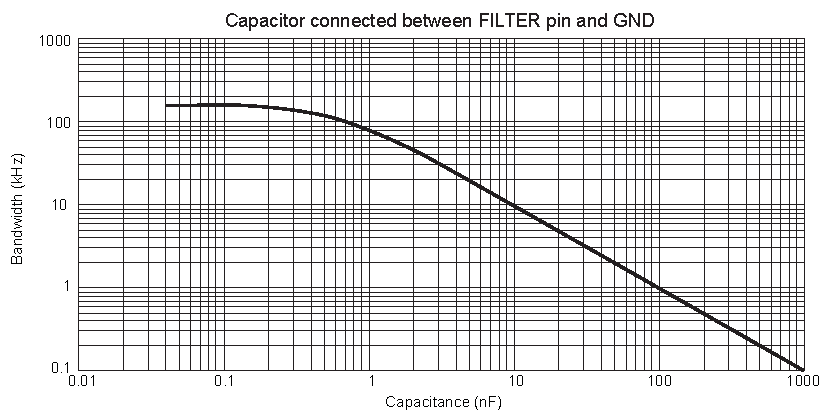
\includegraphics[width=0.5\textwidth]{acs716filter}
	\caption{ACS716 Bandwidth versus External Capacitor Value, $C_F$\protect\footnotemark}
	\label{fig:filter}
\end{figure}
\footnotetext{From ACS716 Datasheet pg 10 http://www.allegromicro.com/\textasciitilde/media/Files/Datasheets/ACS716-Datasheet.ashx} 
\subsection{Overcurrent Threshold}
The overcurrent threshold voltage allows us to detect if the current level is above a user-set limit, likely because of a short. The overcurrent limit is set using a voltage divider composed of $R_H$ and $R_L$ to set a reference voltage on pin $V_{OC}$. When the current through the current path is detected to be higher than 
\[C_{OC} = I_{OC}*37mV/A\] 
the ACS716 drives the output of the FAULT pin high. We chose to set the current threshold at 30A. 
\[C_{OC} = 30A*37mV/A=1.1V\] 
Resistors values of $R_H=2k$ and $R_L=1k$ set $V_{OC}$ at 
\[V_{OC} = 3.3V*\frac{1k}{1k+2k}=1.1V\]
To prevent the fault detection from triggering because of noise a capacitor is connected between fault and ground. The maximum recomended value of 22nF is used.
In previous iterations this features was configured, but the FAULT pin was not connected to the PIC. The pin is now connected to pin B0 on the PIC.

\section{Wire Gages}
\subsection{Wire Sources}
The standard wire gages on purchased connectors are:
\begin{description}
\item[Orbex Slip Ring 2A:]
AWG26 or AWG28
\item[Sparkfun JST PH Jumper Wire:]
24 AWG
\item[Sparkfun JST SH Jumper Wire:]
28 AWG
\item[Mechatronics Lab Red \& Black]
22 AWG
\item[Nick's stores Red, Blue \& Green]
30 AWG
\item[NxR]
30 AWG Black\\
22 AWG Green\\
16-19 AWG Lime Green\\
22 AWG Black, Blue, Red White, Green, Orange in Grey case\\
16 AWG Blue, Brown Green\\
Unknown AWG Red, Black, White shielded clear\\
22 AWG Striped
\end{description}
\subsection{Wire Requirements}
\textbf{24V Power}\\
\textbf{Current Sensor}\\
\textbf{Main Board 5V Power} 22 AWG Red \& Black\\
\textbf{Secondary Board 5V Power} 22 AWG Red \& Black\\
\textbf{1 LED Power} 30 AWG Red \& Black\\
\textbf{2 LED Power} 30 AWG Red \& Black\\
\textbf{3 LED Power} 30 AWG Red \& Black\\
\textbf{Top Magnet Control} 30 AWG Red, Green, Blue \& Red\\
\textbf{Bottom Magnet Power} 22 AWG Red \& Black\\
\textbf{Top Magnet (Slip Ring)} 28 AWG Red, Yellow \& Black\\
\textbf{Bottom Magnet (Slip Ring)} 28 AWG Red, Yellow \& Black\\
\textbf{Top Magnet Encoder} 30 AWG Black, Red, Green \& Blue\\
\textbf{Bottom Magnet Encoder} 30 AWG Black, Red, Green \& Blue\\
\textbf{Motor Encoder} 30 AWG Black, Red, Green \& Blue\\
\textbf{I2C} 30 AWG Green \& Blue\\


\newpage
\section{PCB Bill of Materials}
\begin{longtable}{| >{\centering\arraybackslash}p{0.4\textwidth} | c | l |}
\hline 
\textbf{ Part Number} & \textbf{Quantity} &\textbf{Description}\\ \endhead  \hline
\multicolumn{3}{|l|} {\textbf{Microcontrollers \& Sensors}}  \\ \hline
PIC1, PIC2 & 2 & \href{http://www.digikey.com/product-detail/en/DSPIC33EP512MC806-I%2FPT/DSPIC33EP512MC806-I%2FPT-ND/2835084}{DSPIC33EP512MC806}\\ \hline
X1 & 1 & \href{https://www.sparkfun.com/products/8665}{XBee Series 1 Wired Antenna}\\ \hline
CS1 & 1 & \href{http://www.digikey.com/product-detail/en/ACS716KLATR-6BB-T/620-1445-1-ND/2890908}{ACS716KLATR-\textbf{6BB}-T Current Sensor}\\ \hline
IMU1, IMU2 & 2 & MPU-9150 (Out of Stock)\\ \hline
& 2 & \href{http://www.digikey.com/product-detail/en/MPU-6000/1428-1005-1-ND/4038006}{MPU-6000 (Replacement)}\\ \hline
MD1 & 1 & \href{http://www.digikey.com/product-detail/en/HIP4086ABZ/HIP4086ABZ-ND/936251}{HIP4086 BLDC Motor Driver}\\ \hline

\multicolumn{3}{|l|} {\textbf{Resistors}}  \\ \hline
R40, R41, R43 & 3 & \href{}{0 ohm} \\ \hline
R70 & 1 & \href{}{3.3 $\Omega$} \\ \hline
R34, R35, R36, R37, R38, R39 & 6 & \href{}{10 $\Omega$} \\ \hline
R25 & 1 & \href{}{22 $\Omega$} \\ \hline
R24 & 1 & \href{}{47 $\Omega$} \\ \hline
R2, R7, R8, R9, R10, R11, R12, R13, R17, R18, R19, R31, R66, R67, R68, R69, R77, R78 & 18 & \href{}{1k $\Omega$} \\ \hline
R1 & 1 & \href{}{2k $\Omega$} \\ \hline
R14, R42, R61, R73  & 4 & \href{}{2.2k $\Omega$} \\ \hline
R16 & 1 & \href{}{10k$\Omega$} \\ \hline
R4, R5, R6 & 3 & \href{}{20k $\Omega$} \\ \hline
R3 & 1 & \href{}{330k $\Omega$} \\ \hline

\multicolumn{3}{|l|} {\textbf{Capacitors}}  \\ \hline
C34, C35, C36, C37, C50, C51, C52, C53, C61 & 9 & \href{}{.01uF 0603} \\ \hline
C1, C11, C12, C13, C21, C22, C25, C26, C28, C29, C31, C32, C33, C38, C40, C41, C42, C43, C54, C55, C56, C57, C59, C60, C62 & 25 & \href{}{.1uF 0603} \\ \hline
C7, C8 & 2 & \href{}{.1uF 0603 25V Rated} \\ \hline
C39 & 1 & \href{}{.1uF 0603 50V Rated} \\ \hline
C6, C46, C47 & 3 & \href{}{.1uF 1206} \\ \hline
C17, C18, C19 & 3 & \href{}{.03uF 0603 16V Rated} \\ \hline
C2 & 1 & \href{}{1nF 0603} \\ \hline
C64 & 1 & \href{}{1uF 1206} \\ \hline
C23, C27 & 2 & \href{}{2.2nF 0603} \\ \hline
C20, C24 & 2 & \href{}{10nF 0603} \\ \hline
C15, C48, C49, C63 & 4 & \href{}{10uF 0603 Polarized} \\ \hline
C5, C30 & 2 & \href{}{10uF 0603} \\ \hline
C14, C44, C45, C58, C65 & 5 & \href{}{10uF 1206} \\ \hline
C66, C67 & 2 & \href{}{10uF 1206} \\ \hline
C4 & 1 & \href{}{22nF 0603} \\ \hline
C9, C10 & 1 & \href{}{22uF 0603 15V Rated} \\ \hline
C3& 1 & \href{}{7nF 0603} \\ \hline

\multicolumn{3}{|l|} {\textbf{Diodes}}  \\ \hline
D1, D2, D3, D4, D5, D7, D8, D9, D10, D11, D12 & 11 & \href{http://www.digikey.com/product-detail/en/ES1B/ES1BFSCT-ND/3042546}{ES1B 100V, 1A}\\ \hline

\multicolumn{3}{|l|} {\textbf{Power Converters}}  \\ \hline
P2 & 1 & \href{http://www.digikey.com/product-search/en?WT.z_header=search_go&lang=en&site=us&keywords=CC10-2405SF-E&x=0&y=0&formaction=on}{24V to 5V DC-DC Converter}\\ \hline
P3 & 1 & \href{http://www.digikey.com/product-search/en?vendor=0&keywords=IFX21004TNV51}{24V to 15V \& 5V Linear Regulator}\\ \hline
P1, P4 & 2 & \href{http://www.digikey.com/product-detail/en/TLV1117LV33DCYR/296-28778-1-ND/2666520}{5V to 3.3V LDO Regulator}\\ \hline
P5 & 1 & \href{http://www.digikey.com/product-detail/en/LM2937IMPX-5.0\%2FNOPB/LM2937IMPX-5.0\%2FNOPBCT-ND/3526931}{15V to 5V Linear Regulator}\\ \hline

\multicolumn{3}{|l|} {\textbf{Digital Isolators}}  \\ \hline
DI2, DI3 & 2 & \href{http://www.digikey.com/scripts/DkSearch/dksus.dll?Detail&itemSeq=147517739&uq=635321171204954916}{1 Channel} \\ \hline 
DI1 & 1 & \href{http://www.digikey.com/product-detail/en/SI8660EC-B-IS1/336-2118-5-ND/2623366}{6 Channel}\\ \hline

\multicolumn{3}{|l|} {\textbf{MOSFETs}}  \\ \hline
1H, 1L, 2H, 2L, 3H, 3L & 6 & \href{http://www.digikey.com/product-detail/en/IRFR3806TRPBF/IRFR3806TRPBFCT-ND/1925534}{IRFR3806}\\ \hline
M1, M2 & 2 & \href{http://www.digikey.com/product-detail/en/SSM3K329R,LF/SSM3K329RLFCT-ND/3522426}{SSM3K329RLFCT-ND, 30V, Logic Level}\\ \hline

\multicolumn{3}{|l|} {\textbf{LEDs}}  \\ \hline
& 12 & 0603 LED\\ \hline

\multicolumn{3}{|l|} {\textbf{Switches \& Buttons}}  \\ \hline
SW1 & 1 & \href{http://www.digikey.com/product-detail/en/MHSS1104/679-1848-ND/1795408}{SPDT Slide Switch}\\ \hline
RESET1, USER1, RESET2, USER2 & 4 & \href{http://www.digikey.com/product-detail/en/MJTP1243/679-2452-ND/1798039}{Momentary, Normally Off, Tactile Switch}\\ \hline

\multicolumn{3}{|l|} {\textbf{Connectors}}  \\ \hline
J1, J6, J7, J8, J9, J14, J15, J20, J21 & 9 & \href{http://www.digikey.com/product-search/en?pv88=2&pv69=367&FV=fff40016%2Cfff802f3&k=jst+ph&mnonly=0&newproducts=0&ColumnSort=0&page=1&stock=1&quantity=0&ptm=0&fid=0&pageSize=25}{JST PH 2pos Right Angle Header}\\ \hline
& 9+ & \href{http://www.digikey.com/product-search/en?s=3742&pv88=2&FV=fff40016%2Cfff802fc&k=jst+ph&mnonly=0&newproducts=0&ColumnSort=0&page=1&stock=1&quantity=0&ptm=0&fid=0&pageSize=25}{JST PH 2pos Housing}\\ \hline
& 5+ & \href{http://www.digikey.com/product-search/en?pv88=2&FV=ffec0c8f%2Cfff40016%2Cfff802f5%2Cfffc01c7%2C1640057&mnonly=0&newproducts=0&ColumnSort=0&page=1&stock=1&quantity=0&ptm=0&fid=0&pageSize=25}{JST KR 2pos IDC}\\ \hline

J4, J13 & 2 & \href{http://www.digikey.com/product-search/en?pv69=367&FV=ffec0e9e%2Cfff40016%2Cfff802f3%2C1600005&k=jst+ph&mnonly=0&newproducts=0&ColumnSort=0&page=1&stock=1&quantity=0&ptm=0&fid=0&pageSize=25}{JST PH 3pos Right Angle Header} \\ \hline
& 2+ & \href{http://www.digikey.com/product-search/en?s=3742&pv88=5&FV=fff40016%2Cfff802fc&k=jst+ph&mnonly=0&newproducts=0&ColumnSort=0&page=1&stock=1&quantity=0&ptm=0&fid=0&pageSize=25}{JST PH 3pos Housing}\\ \hline
& 5+ & \href{http://www.digikey.com/product-search/en?pv88=5&FV=ffec0c8f%2Cfff40016%2Cfff802f5%2Cfffc01c7%2C1640057&mnonly=0&newproducts=0&ColumnSort=0&page=1&stock=1&quantity=0&ptm=0&fid=0&pageSize=25}{JST KR 3pos IDC}\\ \hline

J2, J17, J18 & 3 & \href{http://www.digikey.com/product-search/en?pv69=367&FV=ffec0e9e%2Cfff40016%2Cfff802f3%2C1600006&k=jst+ph&mnonly=0&newproducts=0&ColumnSort=0&page=1&stock=1&quantity=0&ptm=0&fid=0&pageSize=25}{JST PH 4pos Right Angle Header} \\ \hline
& 2 & \href{http://www.digikey.com/product-search/en?s=3742&pv88=6&FV=fff40016\%2Cfff802fc&k=jst+ph&mnonly=0&newproducts=0&ColumnSort=0&page=1&stock=1&quantity=0&ptm=0&fid=0&pageSize=25}{JST PH 4pos Housing}\\ \hline
& 5+ & \href{http://www.digikey.com/product-search/en?pv88=6&FV=ffec0c8f%2Cfff40016%2Cfff802f5%2Cfffc01c7%2C1640057&mnonly=0&newproducts=0&ColumnSort=0&page=1&stock=1&quantity=0&ptm=0&fid=0&pageSize=25}{JST KR 4pos IDC}\\ \hline

J3, J12 & 2 & \href{http://www.digikey.com/product-search/en?pv69=367&FV=ffec0e9e%2Cfff40016%2Cfff802f3%2C160001a&k=jst+ph&mnonly=0&newproducts=0&ColumnSort=0&page=1&stock=1&quantity=0&ptm=0&fid=0&pageSize=25}{JST PH 8pos Right Angle Header} \\ \hline
& 2 & \href{http://www.digikey.com/product-search/en?s=3742&pv88=26&FV=fff40016%2Cfff802fc&k=jst+ph&mnonly=0&newproducts=0&ColumnSort=0&page=1&stock=1&quantity=0&ptm=0&fid=0&pageSize=25}{JST PH 8pos Housing}\\ \hline
& 2 & \href{http://www.digikey.com/product-search/en?s=3215&pv88=26&FV=fff40016%2Cfff802f5&k=jst+kr&mnonly=0&newproducts=0&ColumnSort=0&page=1&stock=1&quantity=0&ptm=0&fid=0&pageSize=25}{JST PH 8pos IDC}\\ \hline

& 40+ & \href{http://www.digikey.com/product-detail/en/SPH-001T-P0.5L/455-2147-1-ND/1634655}{JST PH Contact 22-26AWG}\\ \hline
& 40+ & \href{http://www.digikey.com/product-detail/en/SPH-002T-P0.5S/455-1127-1-ND/527358}{JST PH Contact 24-30AWG}\\ \hline
& 40+ & \href{http://www.digikey.com/product-detail/en/SPH-004T-P0.5S/455-1318-1-ND/608807}{JST PH Contact 28-32AWG}\\ \hline

J10, J11, J16, J19 & 4 & \href{http://www.digikey.com/product-detail/en/SM02B-SRSS-TB(LF)(SN)/455-1802-1-ND/926873}{JST SH/SR 2pos Right Angle Header}\\ \hline
& 4+ & \href{http://www.digikey.com/product-search/en/connectors-interconnects/rectangular-connectors-free-hanging-panel-mount/1442549?k=02sr}{JST SR 2pos IDC}\\ \hline
J5 & 1 & \href{http://www.digikey.com/product-detail/en/SM05B-SRSS-TB(LF)(SN)/455-1805-1-ND/926876}{JST SH/SR 5pos Right Angle Header}\\ \hline
& 1 & \href{http://www.digikey.com/product-search/en?pv88=24&FV=ffec0cc3\%2Cfff40016%2Cfff802f5&mnonly=0&newproducts=0&ColumnSort=0&page=1&stock=1&quantity=0&ptm=0&fid=0&pageSize=25}{JST SR 5pos IDC}\\ \hline
& 20+ & \href{http://www.digikey.com/product-detail/en/SSH-003T-P0.2/455-1561-1-ND/720818}{JST SH Contacts 28-32AWG}\\ \hline

JP1, JP2, JP3, JP4, JP5 & 5 & \href{http://www.digikey.com/product-detail/en/0039300020/WM21351-ND/930320}{Molex Mini Fit Jr. 2pos Right Angle Header}\\ \hline
 & 5 & \href{http://www.digikey.com/product-detail/en/0039293026/WM3843-ND/2002650}{Molex Mini Fit Jr. 2pos Vertical Header}\\ \hline
 & 5 & \href{http://www.digikey.com/product-detail/en/0039012020/WM3700-ND/61315}{Molex Mini Fit Jr. 2pos Housing}\\ \hline
 
JP6 & 1 & \href{http://www.digikey.com/product-detail/en/0039303035/WM18446-ND/300079}{Molex Mini Fit Jr. 3pos Right Angle Header}\\ \hline
 & 1 & \href{http://www.digikey.com/product-detail/en/0039012020/WM3700-ND/61315}{Molex Mini Fit Jr. 3pos Housing}\\ \hline
 & 15 & \href{http://www.digikey.com/product-detail/en/0039000077/WM3112CT-ND/1643460}{Molex Mini Fit Jr. Contacts 16AWG}\\ \hline
 & 15 & \href{http://www.digikey.com/product-detail/en/0039000038/WM2501CT-ND/467978}{Molex Mini Fit Jr. Contacts 18-24AWG}\\ \hline
 & 15 & \href{http://www.digikey.com/product-detail/en/0039000046/WM2503CT-ND/3028710}{Molex Mini Fit Jr. Contacts 22-28AWG}\\ \hline
 
 \multicolumn{3}{|l|} {\textbf{Miscellaneous}}  \\ \hline
 & 10 & \href{http://www.keyelco.com/product.cfm/Thru-Hole-Mount/1043P/product_id/13958}{18650 Battery Holder}\\ \hline

\end{longtable}
\section{Board Issues}
Triangles on programming pins
DC-DC Converter
	RC Pin shorted to 24V, should be shorted to GND.
	Pads for standoffs misaligned.
Motor Board Current Sense and Input Voltage mislabeled
On 8 pin connector between PIC board and motor board 3.3V and GND are reversed in order
Motor hall effect sensors connection pins are labeled in reverse order
RDEL is not connected to 15V. 
Encoder inputs are in different order on different boards
Magnet MOSFET - "SOT23F" label is the footprint, part number is actually SSM3K329R
SCL and SDA on secondary board labeled incorrectly
\end{document}
